\section{Model Averaging and Selection}\label{sec:Models}

Our first approach to uncertainty reduction in dMRI tractography \added{(Fig. \ref{fig:base_overview})} addresses the model uncertainty that arises from having to select the rank $r$ in Eq.~(\ref{eq:low-rank}). Underestimating $r$ will miss important fiber directions, while overestimating it confounds the tracking with spurious directions and increases the variance of the true fiber estimates. We approach this choice using Bayesian model comparison in Section~\ref{sec:model-comparison}, and derive the model averaging and model selection approaches from it in Section~\ref{sec:computing-tracking-directions}.

\subsection{Model Comparison in a Bayesian Framework}
\label{sec:model-comparison}
\begin{figure*}[t]
	\centering
	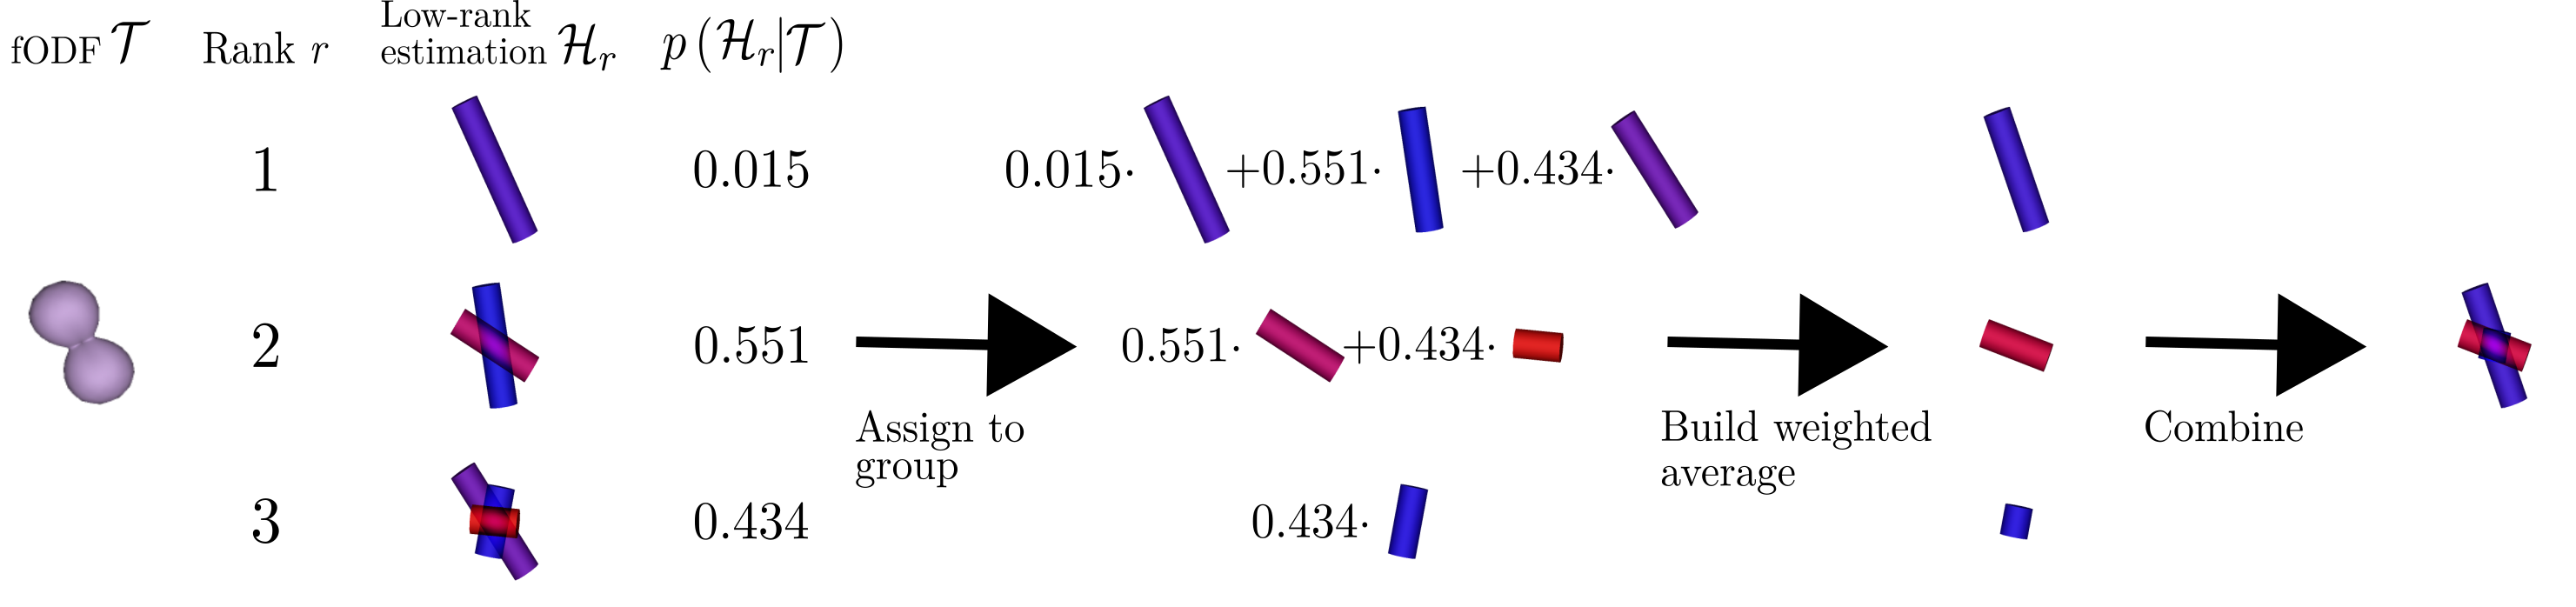
\includegraphics[width=\linewidth]{base_overview_scheme}
	\caption{\added{Computation of tracking directions via model averaging. For a given fODF $\mathcal{T}$, low-rank approximations with ranks $r \in \left\{ 1,2 , 3 \right\}$ are computed and their probabilities evaluated using the Bayesian framework described in Section \ref{sec:model-comparison}. The directions of the approximations are then aligned before an average is taken that minimizes the overall sum of angles between the resulting
weighted means $\mathbf{v}_i$ and their corresponding $\mathbf{v}_i^{\left( r
\right)}$. The final model is a sum of the three models weighted by posterior probability $p \left( \mathcal{T} \mid \mathcal{H}_r \right)$, as shown in Section \ref{sec:computing-tracking-directions}.}}
	\label{fig:base_overview}
\end{figure*}
In Bayesian model comparison, we are interested in the
posterior probability $p \left( \mathcal{H}_r \mid \mathcal{T} \right)$, where
$\mathcal{H}_r$ denotes the hypothesis that extracting $r$ fibers is optimal for a given fODF $\mathcal{T}$. Using Bayes' theorem of
conditional probability, the posterior probability can be rewritten as
\begin{align}
	p \left( \mathcal{H}_r \mid \mathcal{T} \right) \propto p \left(
		\mathcal{T} \mid \mathcal{H}_r 
	\right) p \left(  \mathcal{H}_r \right), 
	\label{eq:Bayes}
\end{align}
where \added{the common normalizing factor can be omitted when taking ratios of $p \left( \mathcal{H}_r \mid \mathcal{T} \right)$ for different $r$, and}
$p \left(  \mathcal{H}_r \right)$ is our prior belief that rank $r$ is
suitable, without considering the fODF. Since literature values for the prevalence of different $r$ over the white matter vary  \cite{BEHRENS2007144,Jeurissen:2012, Schultz:MICCAI12}, we use a
non-informative prior that assigns equal prior probability to the values of $r
\in \left\{ 1,2,3 \right\}$. The case $r=0$ can be excluded since we limit
tracking to a white matter mask. 

The factor $p \left( \mathcal{T} \mid \mathcal{H}_r \right)$ is the
probability of the fODF $\mathcal{T}$ given a rank $r$. In the context of
Bayesian model comparison, it is referred to as model evidence. It is derived from $p
\left( \mathcal{T} \mid \mathcal{H}_r , \Theta_r \right)$, the posterior
probability of $T$ given an $r$-fiber model with a specific parameter vector
$\Theta_r$. In our case, $\Theta_r$ contains the variables from Eq.
(\ref{eq:low-rank}), i.e., $\Theta_r \coloneqq \left( \lambda_1 , \mathbf{v}_1 , \dots
, \lambda_r , \mathbf{v}_r \right)$. 

The overall model evidence is obtained by marginalization over parameter values,
\begin{align}
	p \left( \mathcal{T} \mid \mathcal{H}_r \right) = \int p \left(
		\mathcal{T} \mid \mathcal{H}_r , \Theta_r 
	\right) p \left( \Theta_r \mid \mathcal{H}_r  \right) d \Theta_r. 
	\label{eq:model-evidence}
\end{align}

Since a direct calculation of Eq. (\ref{eq:model-evidence}) would require solving a
high dimensional integral, we use an approximation via the Bayesian Information
Criterion
\[ \text{BIC} = k \ln \left( n \right) - 2 \ln \left( p \left( \mathcal{T} \mid
\mathcal{H}_r, \hat{\Theta}_r \right) \right), \]
where $p \left(  \mathcal{T} \mid \mathcal{H}_r , \hat{\Theta}_r \right)$
corresponds to the likelihood of the rank-$r$ with parameters $\hat{\Theta}_r$
that best fit the fODF $\mathcal{T}$, $k$ is the number of parameters in
$\Theta_r$, and $n$ denotes the number of data points to which the model was
fitted \cite{Schwarz1978}. We note that $k=3r$ increases with $r$, which penalizes the choice of multiple fibers, unless it leads to a sufficient increase of $p \left(  \mathcal{T} \mid \mathcal{H}_r , \hat{\Theta}_r \right)$. Under certain conditions, the BIC is related to the
model evidence by \cite{Konishi2008}
\begin{align}
	p \left( \mathcal{T} \mid \mathcal{H}_r \right) \approx \exp \left(  -
		\frac{\text{BIC}}{2}
\right).
	\label{eq:BIC-model}
\end{align}

% \subsection{From Model Likelihood to Model Uncertainty}
This allows us to compute the model evidence in a simple and efficient way.
However, we still need to provide an equation for $p
\left( \mathcal{T} \mid \mathcal{H}_r , \hat{\Theta}_r \right)$. Therefore, we
use the relative magnitude of the corresponding low-rank approximation residual 
\begin{align}
	\| \tilde{\mathcal{R}}^{\left( r \right)} \| = \frac{ \| \mathcal{T} -
	\mathcal{T}^{\left( r \right)} \| }{ \| \mathcal{T} \|} \in \left[ 0,1
	\right],
	\label{eq:residual}
\end{align}
since a smaller residual from a rank-$r$ approximation should indicate a higher probability of $\mathcal{T}$ being a perturbation of a rank-$r$ tensor. Since many factors contribute to the magnitude of this residual, including measurement noise, fiber spread, and inaccuracies in the convolution kernel, we pragmatically model
$p
\left( \mathcal{T} \mid \mathcal{H}_r , \hat{\Theta}_r \right)$ with the computationally efficient Kumaraswamy Probability Density Function (PDF) \cite{Kumaraswamy1980}
\begin{align}
	f \left( x, a, b \right) \coloneqq ab x^{a-1} \left( 1- x^a
	\right)^{b-1} \text{ for } x \in \left( 0,1 \right) \text{ and } a,b >
	0
	\label{eq:Kumaraswamy}
\end{align}
which is defined on the correct interval $(0,1)$, and can be tuned to achieve the correct qualitative behavior of decreasing with increasing $\| \tilde{\mathcal{R}}^{\left( r \right)} \|$, at an empirically plausible slope.

As illustrated in \cite{Gruen:2021}, setting $a=1$, $b=20$ leads to a fraction of two and three fiber voxels that matches estimates from the literature, and to the detection of single fiber voxels in regions that are widely assumed to contain a single dominant orientation.

\subsection{Computing Tracking Directions from Alternative Models}
\label{sec:computing-tracking-directions}

As in our previous work \cite{Gruen:2021}, we fuse the information from tensor
approximations with different ranks $r \in \left\{ 1,2 , 3 \right\}$ by taking a weighted sum of the
corresponding parameters $\mathbf{v}_i^{\left( r \right)}$ and
$\lambda_i^{\left( r \right)}$ with weights given by the above-defined posterior probabilities. We refer to this strategy as \emph{model averaging.}

Before computing the weighted sum, we have to establish a correspondence between the directions of the
different $r$-fiber models. In other words, we have to re-order the directions from each rank $r$ such that the first directions of the two- and three-fiber models are matched with the direction from the single fiber model, and that the second directions of the two- and three-fiber models match. This leads to $2! \times 3! =12$ possible assignments, from which we
select the one that minimizes the overall sum of angles between the resulting
weighted means $\mathbf{v}_i$ and their corresponding $\mathbf{v}_i^{\left( r
\right)}$.

Previous tractography algorithms that were based on low-rank tensor approximation \cite{Ankele:CARS2017} used a different strategy, that we refer to as \emph{model selection:} They determined an optimal rank $r \in \left\{ 1, \added{2}, 3 \right\}$ in each integration step and used the resulting set of
directions $\mathbf{v}_i$ for tracking. In cases where several ranks have non-negligible probabilities, this introduces an uncertainty that model averaging aims to reduce. We include this approach
as a baseline in our experiments. To enable a direct comparison, we select the model with the highest probability $p \left(
 \mathcal{H}_r \mid \mathcal{T} \right)$ according to the same Bayesian framework.
 

%%% Local Variables:
%%% mode: latex
%%% TeX-master: "../main"
%%% End:
